\documentclass[10pt]{beamer}

\usetheme{CambridgeUS}
\usepackage[english, russian]{babel}
\usepackage[utf8]{inputenc}
\usepackage{caption}
\usepackage{etoolbox}
\usepackage{multicol}
\usepackage{listings}
\usepackage{wasysym}
\usepackage{mathtools}
\DeclarePairedDelimiter\ceil{\lceil}{\rceil}
\DeclarePairedDelimiter\floor{\lfloor}{\rfloor}

\definecolor{mygreen}{rgb}{0,0.6,0}
\lstset{
  basicstyle=\ttfamily\footnotesize,        % the size of the fonts that are used for the code
  breaklines=true,                 % automatic line breaking only at whitespace
  captionpos=b,                    % sets the caption-position to bottom
  commentstyle=\color{mygreen},    % comment style
  keywordstyle=\color{blue},       % keyword style
  stringstyle=\color{red},     % string literal style
  showstringspaces=false,
  morekeywords={include, printf},
  texcl=true     %<---- added
}

\title[\href{https://goo.gl/NRgp8K}{https://goo.gl/NRgp8K} (Term 3)]{Декартово дерево по неявному ключу}
\author[Гусев Илья, Булгаков Илья]{Гусев Илья, Булгаков Илья}
\institute[МФТИ] 
{Московский физико-технический институт\\*}
\date{Москва, 2019}
\subject{Computer Science}

\begin{document}

\begin{frame}
  \titlepage
\end{frame}

\begin{frame}{Содержание}
\tableofcontents
\end{frame}

\section{Декартово дерево: повторение}
\begin{frame}[fragile]{Декартово дерево: повторение}
\begin{itemize}
    \item Бинарное дерево поиска по ключу x
    \item Куча по приоритету y
    \item В одной вершине храним x и y
    \item Случайные приоритеты $\rightarrow$ балансировка
\end{itemize}
\end{frame}

\begin{frame}[fragile]{Декартово дерево}{Внутрненние операции}
\begin{itemize}
    \item Merge - склейка 2 деревьев; все ключи одного меньше всех ключей другого: в среднем $O(log(N))$
    \item Split - разрезание по ключу на 2 дерева: в среднем $O(log(N))$
\end{itemize}
\end{frame}

\subsection{Merge}
\begin{frame}[fragile]{Декартово дерево}{Merge}
\begin{center}
    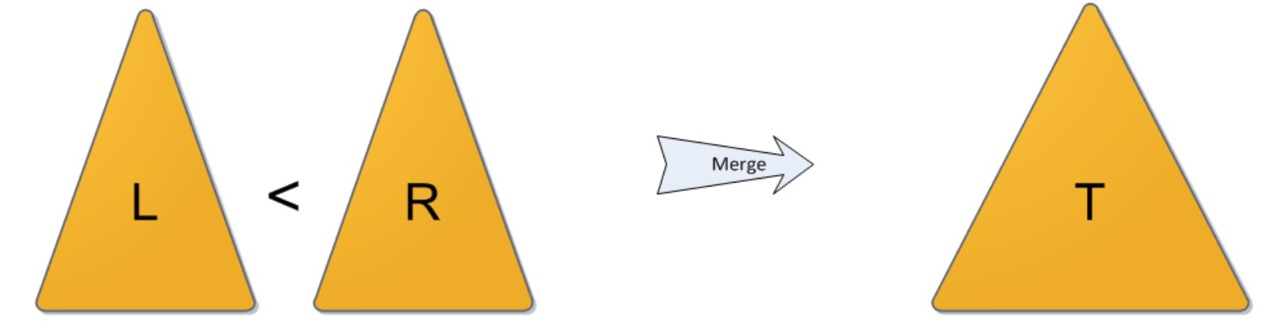
\includegraphics[width=12cm, height=3cm]{Term_1/Source/Pirctures/treap_merge.jpg}\\
\end{center}
\begin{itemize}
    \item Все ключи дерева L меньше ключей дерева R
    \item Б.о.о. приоритет (y) корня левого дерева больше приоритета корня правого дерева $\rightarrow$ новый корень - корень левого дерева
\end{itemize}
\end{frame}

\begin{frame}[fragile]{Декартово дерево}{Merge}
\begin{center}
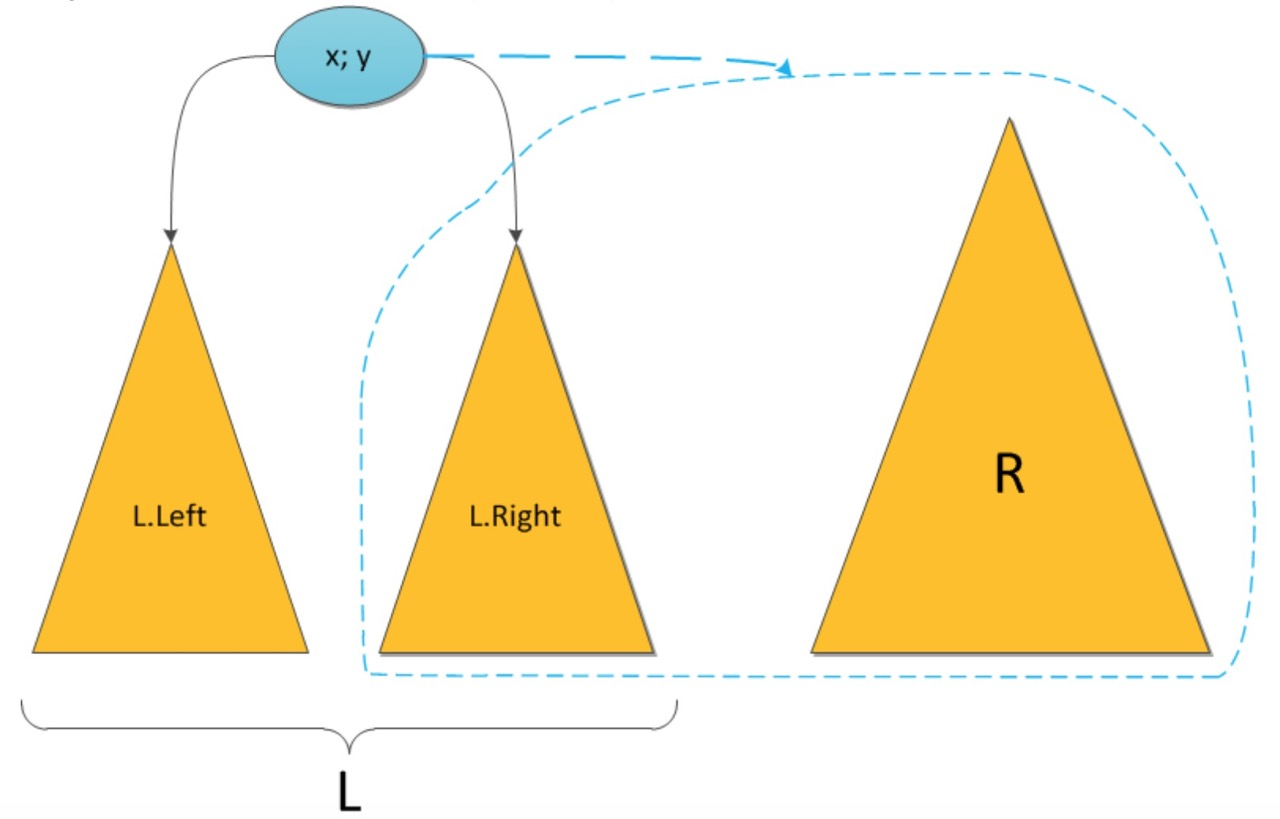
\includegraphics[width=8cm, height=4cm]{Term_1/Source/Pirctures/treap_merge_step.jpg}
\end{center}
\begin{itemize}
    \item Тогда R - точно в правом поддереве нового корня
    \item L.Left -  точно левое поддерво нового корня
    \item Рекурсивно сливаем L.Right и R
    \item База рекурсии: хотя бы одно дерево пустое
\end{itemize}
\end{frame}

\begin{frame}[fragile]{Декартово дерево}{Merge}
\begin{itemize}
    \item Сложность: сумма высот деревьев, в среднем $O(log(n) + log(m))$
\end{itemize}
\end{frame}

\subsection{Split}
\begin{frame}[fragile]{Декартово дерево}{Split}
\begin{center}
    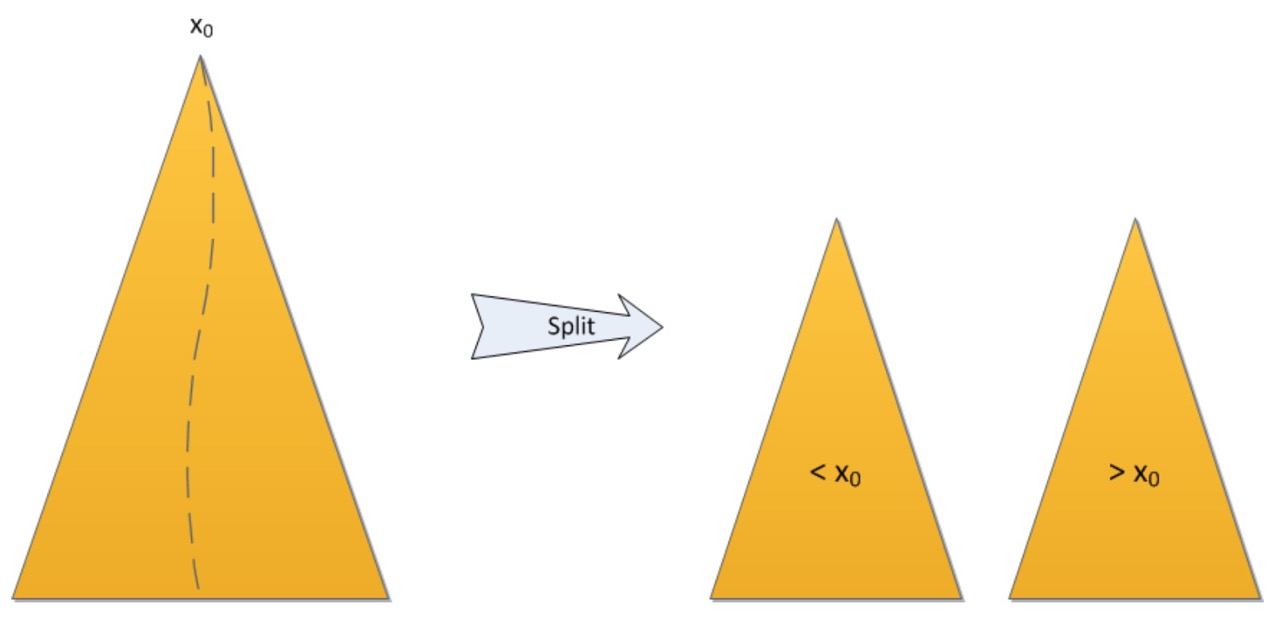
\includegraphics[width=10cm, height=4cm]{Term_1/Source/Pirctures/treap_split.jpg}\\
\end{center}
\begin{itemize}
    \item Разделяем по ключу $x_o$
    \item Б.о.о ключ корня меньше $x_0$
\end{itemize}
\end{frame}

\begin{frame}[fragile]{Декартово дерево}{Split}
\begin{center}
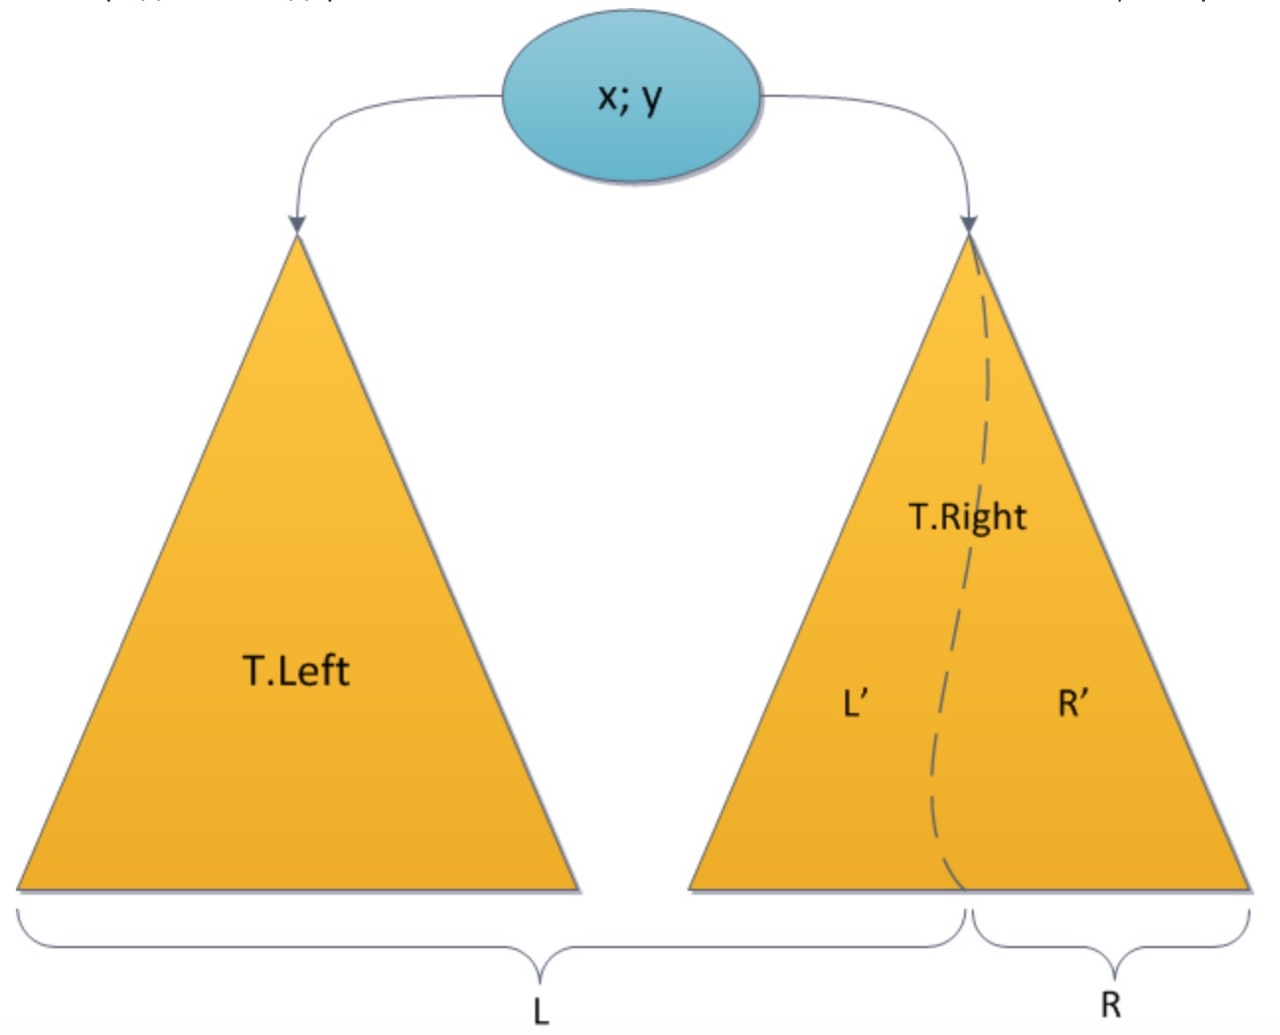
\includegraphics[width=6cm, height=4.5cm]{Term_1/Source/Pirctures/treap_split_step.jpg}
\end{center}
\begin{itemize}
    \item Рекурсивно делим правое поддерво корня на L' и R'
    \item L' - новое правое поддерво корня
\end{itemize}
\end{frame}

\begin{frame}[fragile]{Декартово дерево}{Split}
\begin{itemize}
    \item Сложность: высота изначального дерева, в среднем $O(log(n))$
\end{itemize}
\end{frame}

\subsection{Insert}
\begin{frame}[fragile]{Декартово дерево}{Insert}
\begin{center}
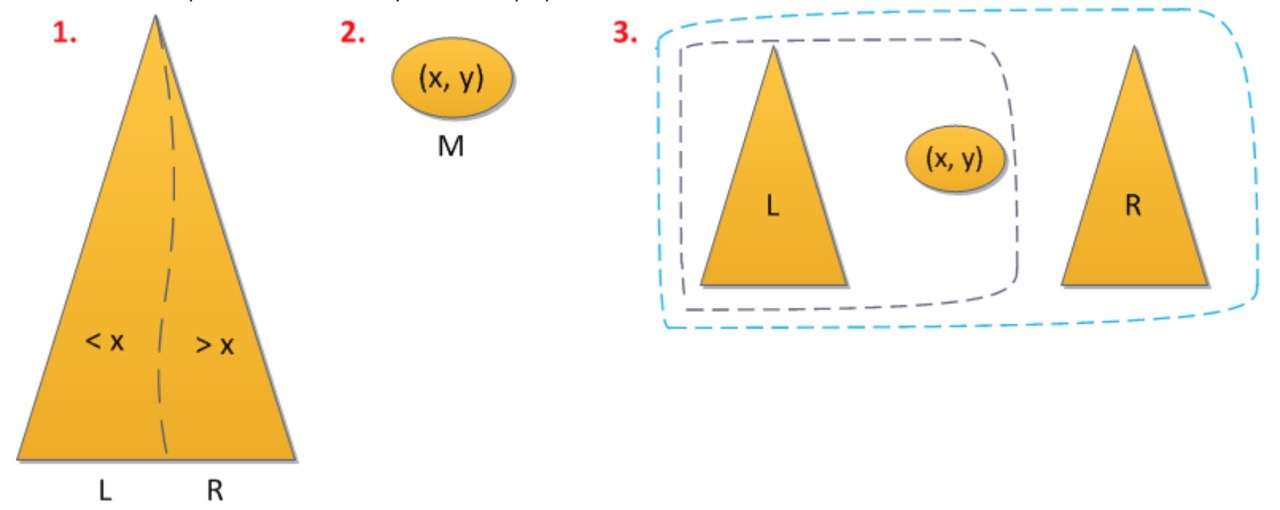
\includegraphics[width=12cm, height=4.5cm]{Term_1/Source/Pirctures/treap_insert.jpg}\\
Вставка элемента  (x, y)\\
1 Split + 2 Merge
\end{center}
\end{frame}

\subsection{Remove}
\begin{frame}[fragile]{Декартово дерево}{Remove}
\begin{center}
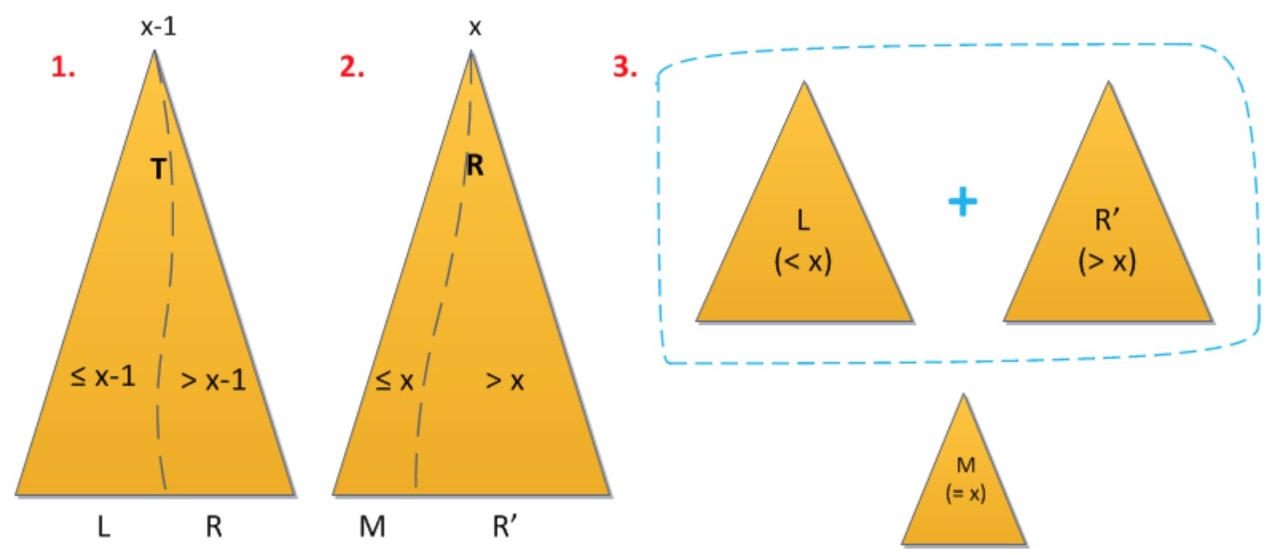
\includegraphics[width=12cm, height=4.5cm]{Term_1/Source/Pirctures/treap_remove.jpg}\\
Удаление элементов с ключом x\\
2 Split + 1 Merge
\end{center}
\end{frame}

\section{Декартово дерево по неявному ключу}
\begin{frame}[fragile]{Декартово дерево по неявному ключу}
Декартово дерево - бинарное дерево поиска слева направо и куча сверху вниз\\
Неявный ключ - количество элементов в нашей структуре, находящихся левее нашего элемента\\
Эквивалентное определение:
\begin{itemize}
    \item Корнем дерева является элемент массива, имеющий минимальное значение A, скажем A[i]
    \item Левым поддеревом является декартово дерево по неявному ключу на массиве A[1..i-1]
    \item Правым поддеревом является декартово дерево по неявному ключу на массиве A[i+1..N]
\end{itemize}
\end{frame}

\begin{frame}[fragile]{Изменения в операциях}
\begin{itemize}
    \item Merge не меняется
    \item Split делается через поддержание размера поддеревьев
    \item Insert не меняется $\rightarrow$ вставка в массив за O(log(n))
    \item Remove не меняется $\rightarrow$ удаление из массива за O(log(n))
\end{itemize}
\end{frame}

\appendix

\begin{frame}[allowframebreaks]
  \frametitle<presentation>{Полезные ссылки}
    
  \begin{thebibliography}{10}
{
  \beamertemplatebookbibitems
  % Start with overview books.

  \bibitem{neercwiki}
  \texttt{Викиконспекты: Декартово дерево по неявному ключу}
  \newblock \href{http://bit.ly/2VTDSwp}
  {\texttt{http://bit.ly/2VTDSwp}}
  
  \bibitem{emaxx}
  \texttt{Emaxx: Неявные декартовы деревья}
  \newblock \href{http://www.e-maxx-ru.1gb.ru/algo/treap}
  {\texttt{http://www.e-maxx-ru.1gb.ru/algo/treap}}
  
  \bibitem{habr}
  \texttt{Хабр: Декартово дерево: Часть 3. Декартово дерево по неявному ключу}
  \newblock \href{https://habr.com/ru/post/102364/}
  {\texttt{https://habr.com/ru/post/102364/}}
}
  \end{thebibliography}
  \end{frame}

\end{document}


